\documentclass[11pt]{report}            % Report class in 11 points
\parindent0pt  \parskip10pt             % make block paragraphs
\raggedright                            % do not right-justify
\usepackage{amsmath, amssymb, amsthm,graphicx, enumitem, hyperref,gensymb, float} %, threeparttable}
\newcommand{\ro}{\mathcal{R}_0}
\makeatletter
\newcommand*{\centerfloat}{%
  \parindent \z@
  \leftskip \z@ \@plus 1fil \@minus \textwidth
  \rightskip\leftskip
  \parfillskip \z@skip}
\makeatother
%*******************************************************************%
\title{\bf Mayo Case Study Rough Draft\\
\large Using Discrete Event Simulation}  % Supply information
\author{Justin Hood\\
MSCS 791}              %   for the title page.
\date{\today}                           %   Use current date.
\begin{document}                        % End of preamble, start of text.
\maketitle                              % Print title page.
\pagenumbering{roman}                   % roman page number for toc
\setcounter{page}{2}                    % make it start with "ii"
\tableofcontents                        % Print table of contents
\newpage
\section*{Abstract}
\addcontentsline{toc}{section}{Abstract}

\section*{Introduction}                % Print a "chapter" heading\
\addcontentsline{toc}{section}{Introduction}
\pagenumbering{arabic}                  % Start text with arabic 1
In this case study, we are tasked with both modeling and optimizing the workflow for a pharmacy based on a sample of data regarding task duration and incoming order frequency. In addition to the sample data for the pharmacy, we are also given a brief overview of the basic workflow for the pharmacy. Using this information, we shall begin by constructing a discrete event simulation in c++ to test our so called ``control" case, i.e. the pharmacy described by the basic information. Once this simulation is running and tested, we shall attack the optimization on two fronts.
\begin{enumerate}
\item Optimizing task priority within the workflow (Picking the best queue to pull from)
\item Optimizing staff breakdown (Best number of pharmacists vs. technicians to employ)
\end{enumerate}
\section*{Methods}
\addcontentsline{toc}{section}{Methods}
In order to effectively model and optimize the workflow in this pharmacy, we 

\subsection*{Process Workflow}
\addcontentsline{toc}{subsection}{Process Workflow}
To begin, we consider the basic workflow. As stated, due to regulations, pharmacists are able to perform tasks that technicians are unable to. The task breakdown is as follows:
\begin{center}
\begin{tabular}{|c||c|}
\hline
Technician & Pharmacist\\\hline\hline
Order Entry & Order Entry \\\hline
& Entry Verification \\\hline
Drug Preparation & Drug Preparation\\\hline
& Preparation Verification\\\hline
Distribution & Distribution\\\hline
\end{tabular}
\end{center}
This is to say that $T_{Technician}\subset T_{Pharmacist}$.  With this distinction in mind, we consider the flowchart contained in Figure \ref{fig:flowchart}, which describes the process workflow graphically.
\begin{figure}[H]
\centering
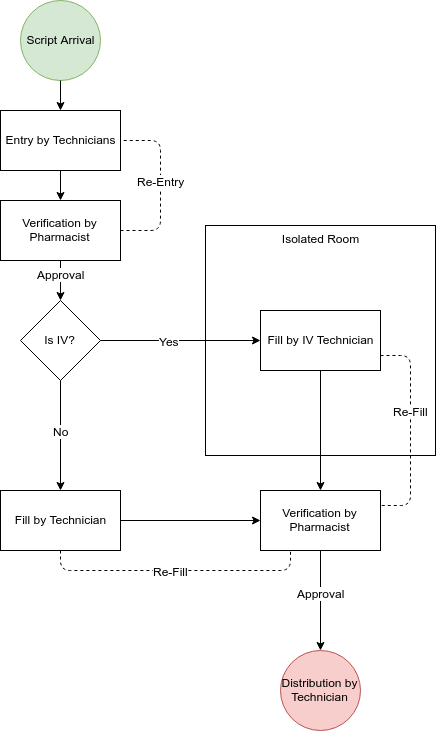
\includegraphics[scale=.5]{Flowchart.png}
\caption{Pharmacy workflow by task position noting which tasks are pharmacist only.}
\label{fig:flowchart}
\end{figure}
Here we may clearly see that with the exception of the IV Fill step, the workflow is fairly linear, which will make the simulation fairly simple to write. The basic workflow is:
\begin{enumerate}
\item Order comes in and enters the Entry Task Queue
\item Employee enters the order, order enters the Entry Verification Queue
\item Pharmacist verifies the entry, order enters the Fill Queue
\item Employee fills the order, order enters the Fill Verification Queue
\item Pharmacist verifies the fill, order enters the Dispense Queue
\item Employee dispenses the order through the window
\end{enumerate}
There is a fork in the process workflow after step 3, where the order's type (Oral vs. IV) must be checked so it may be put in the appropriate filling queue, however this does not affect the linearity of the process at this step. 
%\subsection*{SIR Model}
%\addcontentsline{toc}{subsection}{SIR Model}
%
%\subsection*{Beta}
%\addcontentsline{toc}{subsection}{Beta}
%$\beta$ is a product of many factors, the main being team success, physical locale (weather, population, income), and the social environment of the city\cite{light}. In order to compute a given teams $\beta$ value, we must quantify these factors as follows.
%\subsubsection*{Team Success}
%\addcontentsline{toc}{subsection}{Team Success}
%
%\begin{equation}\label{acoeff}
%\log(a_t) = 14.1 + 0.2205(WINT)+.091\log(POP)-0.3766\log(INC)
%\end{equation}
%\begin{equation}\label{bcoeff}
%\log(b_t) = 9.171 + .03(WINT)+.028\log(POP)-.1879\log(INC)
%\end{equation}
%Each of the coefficients we compute have incredibly large t-values, which aligns with the linear nature of (\ref{a}) and (\ref{b}). As such, we are confident that these coefficients are correct for the purposes of our analysis. With these coefficients computed, we can compute the following location score for our potential Milwaukee team,
%
%\begin{table}[H]
%\centerfloat
%\begin{tabular}{lrrrrrrrr}
%\hline
%\multicolumn{9}{c}{Location Score for Milwaukee} \\
%Team & Population$^a$ & GDP per capita$^b$ & Temperature$^c$ & WINT & $a_t$ & $b_t$ & $H_t$ & $h_t$\\
%\hline
%Milwaukee & 1.572245 & \$58,680.00 & -2 & 1 & 27583.4 & 1274.342 & 117.1288 & 0.9990123
%\end{tabular}
%\caption{$^a$in Millions \cite{population}; $^b$USD \cite{gdp}; $^c$ \degree C \cite{weather}}
%\label{table:Milwaukee_H}
%\end{table}
%
%\end{description}
\begin{thebibliography}{9}
%\bibitem{light} J. Light, A. Chernin, and J. M. Heffernan, ``NHL expansion and fan allegiance: a mathematical modelling study,” \textit{Mathematics-in-Industry Case Studies}, vol. 7, no. 1, Apr. 2016.
%\bibitem{money} M. Ozanian and K. Badenhausen, ``The NHLs Most Valuable Teams” \textit{Forbes}, 21-Feb-2019. [Online]. Available: \url{https://www.forbes.com/sites/mikeozanian/2018/12/05/the-nhls-most-valuable-teams/}. [Accessed: 25-Sep-2019].
%\bibitem{stats}  HockeyDB.com (2019) National Hockey League history and statistics. \url{http://www.hockeydb.com/ihdb/stats/leagues/141.html}. Web
%\bibitem{jones}J. C. H. Jones and D. G. Ferguson, ``Location and Survival in the National Hockey League,” \textit{The Journal of Industrial Economics}, vol. 36, no. 4, p. 443, Jun. 1988.
%\bibitem{population} US Census Bureau and Data Integration Division, ``Population Estimates,” \textit{Metropolitan and Micropolitan Statistical Area Totals Dataset: Population and Estimated Components of Change: April 1, 2010 to July 1, 2014 - U.S Census Bureau}. [Online]. \url{https://web.archive.org/web/20150504102404/http://www.census.gov/popest/data/metro/totals/2014/CBSA-EST2014-alldata.html}. [Accessed: 30-Sep-2019].
%\bibitem{gdp} ``Regional Economic Accounts GDP and Personal Income,” \textit{BEA}. [Online]. \url{https://apps.bea.gov/itable/drilldown.cfm?reqid=70&stepnum=40&Major_Area=5&State=5&Area=XX&TableId=504&Statistic=1&Year=2014&YearBegin=-1&Year_End=-1&Unit_Of_Measure=Levels&Rank=1&Drill=1&nRange=5}. [Accessed: 28-Sep-2019].
%\bibitem{weather} ``Milwaukee Temperatures: Averages by Month,” \textit{Milwaukee WI Average Temperatures by Month - Current Results}. [Online]. \url{https://www.currentresults.com/Weather/Wisconsin/Places/milwaukee-temperatures-by-month-average.php}. [Accessed: 30-Sep-2019].
%\bibitem{whynot} J. Hand, C. Jozwik, H. Magner, Z. Brooke, A. Landowski, A. Parquette, and E. Johnson, ``Why Milwaukee is Not an NHL City,” \textit{Milwaukee Magazine}, 16-Nov-2018. [Online]. \url{https://www.milwaukeemag.com/milwaukee-not-nhl-city/}. [Accessed: 29-Sep-2019].
%\bibitem{draft} ``2017 NHL Expansion Draft,” \textit{Wikipedia}, 27-Apr-2019. [Online]. \url{https://en.wikipedia.org/wiki/2017_NHL_Expansion_Draft}. [Accessed: 29-Sep-2019].
%\bibitem{wisco} ``NHL Players Born in Wisconsin, United States,” \textit{Hockey}. [Online]. \url{https://www.hockey-reference.com/friv/birthplaces.cgi?country=US&province&state=WI&fbclid=IwAR1vb6vzR95-DX0B_zRyV_gLxYcWMneos3Ppn8RBNsnHQqzA9d4sJj4X_aA}. [Accessed: 29-Sep-2019].
\end{thebibliography}
\end{document}                          % The required last line
